% Appendix

\chapter{PLATFORM DEVELOPMENT}

During the development, there were several challenges faced:
\begin{enumerate}
    \item Distribution of the source code;
    \item Distribution of the NUIX-Studio App demos;
    \item Creating Tutorials;
    \item Providing API for external projects;
    \item Updating the dependencies;
    \item Rewriting the code to support new architectures.
\end{enumerate}

The platform's source code is hosted at \cite{NUIXStudio} repository. The source code distribution required keeping the repository size at a minimum while providing an easy installation procedure. NUIX-Studio was shared as a separate package to follow these requirements, possible to integrate into any Unity project.

The prototypes of the NUIX-Studio platform did not initially support Virtual reality (Figure~\ref{fig:Prototype2-figure}) and were based on a different architecture (Figure~\ref{fig:Prototype3Structure-figure}).


\begin{figure}
  \centering
  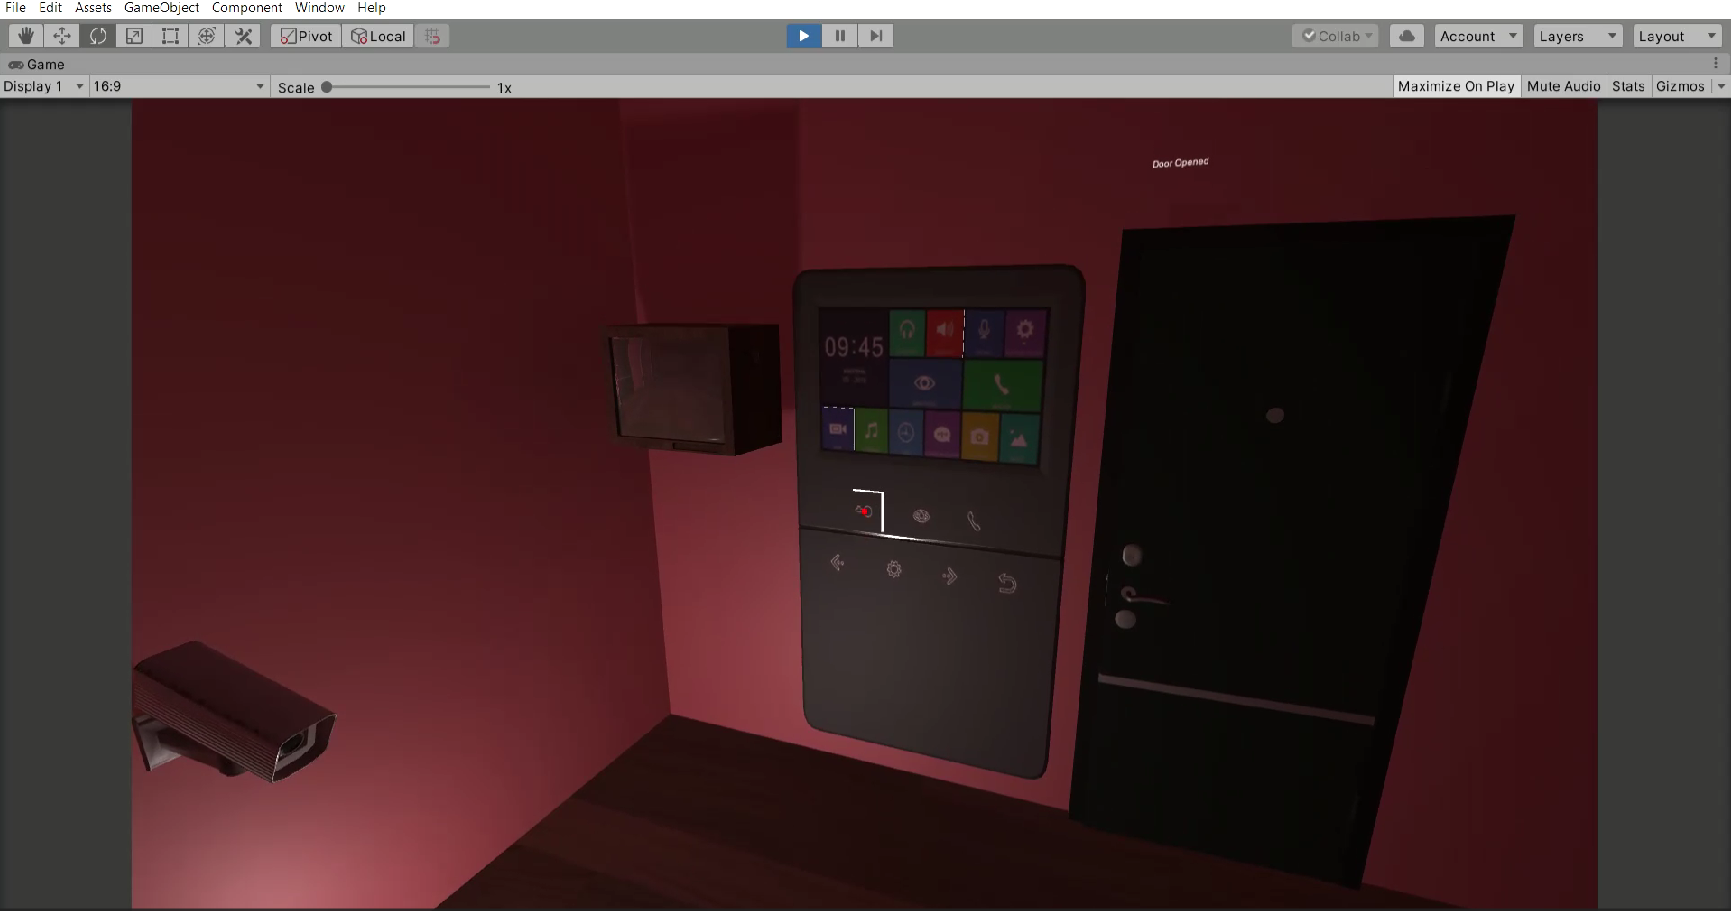
\includegraphics[width=0.6\linewidth]{figures/Prototype2.png}
  \caption{The second prototype of the VR-IoT Research platform}
  \label{fig:Prototype2-figure}
\end{figure}

\begin{figure}
  \centering
  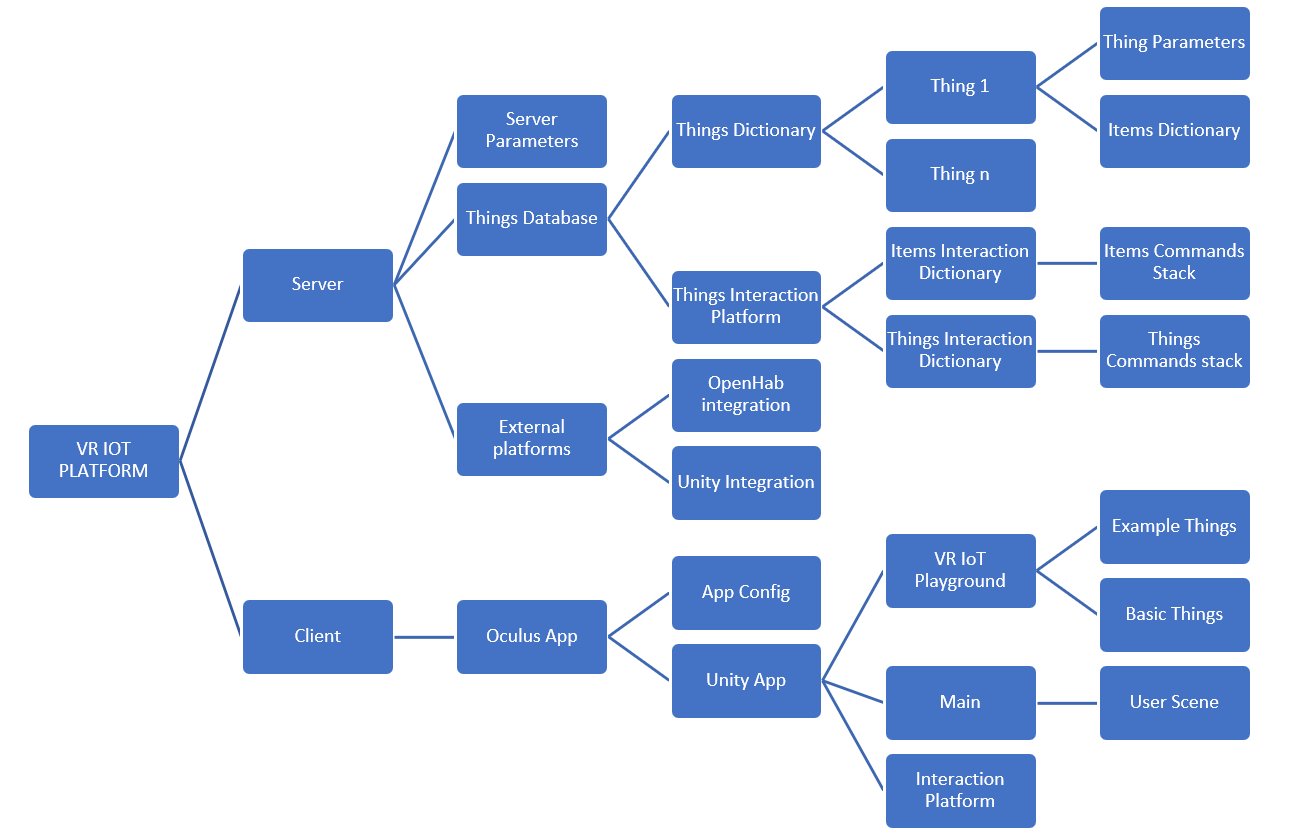
\includegraphics[width=0.9\linewidth]{figures/Prototype3Structure.png}
  \caption{The third prototype's structure}
  \label{fig:Prototype3Structure-figure}
\end{figure}

The final structure used in NUIX-Studio is different from the structure in Figure~\ref{fig:Prototype3Structure-figure}. In the previous prototypes, the server was responsible for storing and synchronizing item parameters and keeping all the Unity-specific functionality in a separate framework. This framework was used to build Item representations for virtual reality and share them to other NUIX-Studio App instances as Unity objects. This approach's main limitation is that Unity objects have a much bigger size than the Data transfer objects used in the final prototype. These Unity objects were synchronized every frame for the simultaneous work, which dramatically dropped the NUIX-Studio App instances' performance.

\begin{figure}
  \centering
  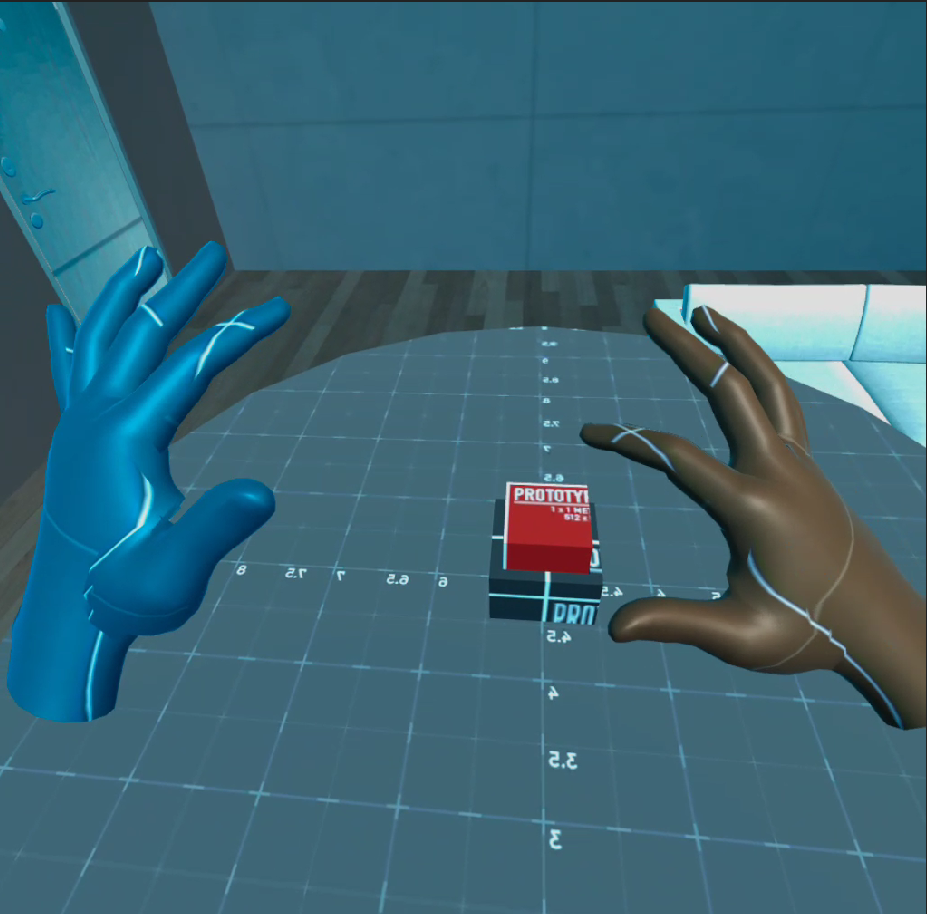
\includegraphics[width=0.6\linewidth]{figures/Prototype3.png}
  \caption{The third prototype of the VR-IoT Research platform. Button Widget.}
  \label{fig:Prototype3-figure}
\end{figure}

The third prototype provided only a button Widget (Figure~\ref{fig:Prototype3-figure}), but after integrating Mixed Reality Toolkit in the fourth prototype (Figure~\ref{fig:Prototype4-figure}), additional Widgets were added to the platform.

\begin{figure}
  \centering
  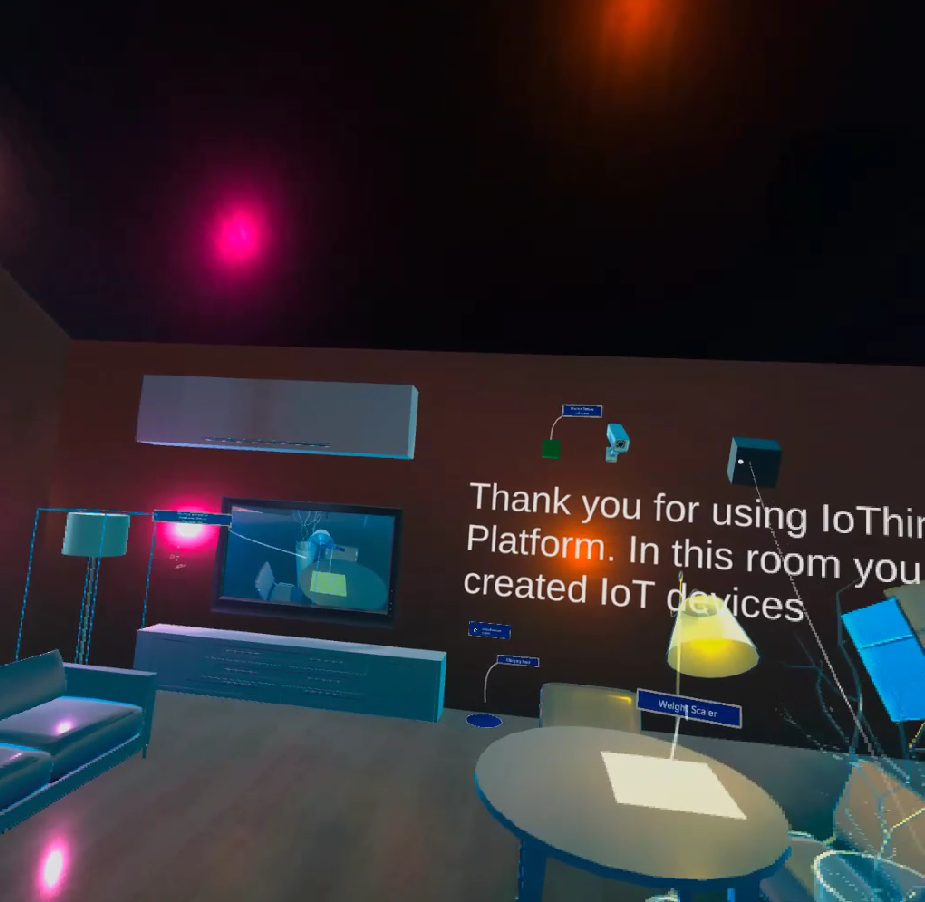
\includegraphics[width=0.6\linewidth]{figures/Prototype4.png}
  \caption{The fourth prototype of the VR-IoT Research platform. A virtual copy of the real-world Smart home environment was used with virtual items added, such as location, contact, player, switch, and dimmer items. Also several Widgets were supported: sight sensor, motor, light widget, pressure sensor, video streaming screens and gesture recognition.}
  \label{fig:Prototype4-figure}
\end{figure}

In the final prototype (Figure~\ref{fig:FinalPrototype-figure}), code for most of the items was rewritten to support the new architecture. 

\begin{figure}
  \centering
  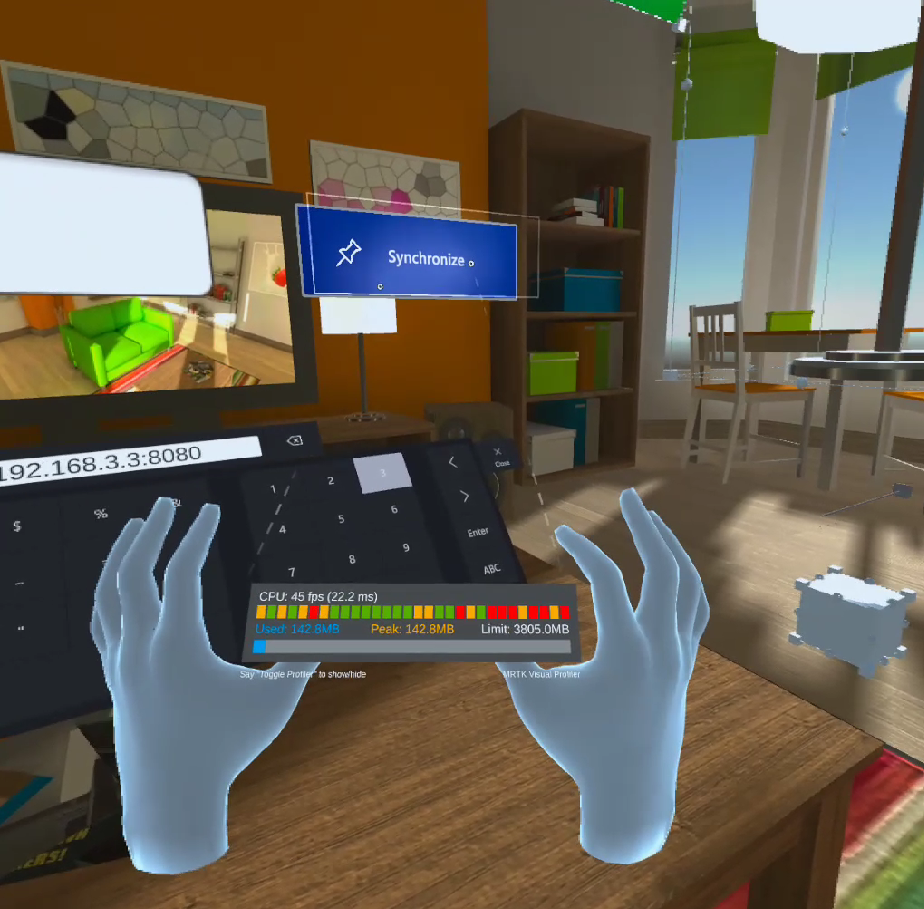
\includegraphics[width=0.6\linewidth]{figures/FinalPrototype.png}
  \caption{Screenshot of the final prototype of NUIX-Studio.}
  \label{fig:FinalPrototype-figure}
\end{figure}